\documentclass[tikz,border=2mm]{standalone}
\usepackage{chessfss}
\usetikzlibrary{matrix,backgrounds}

\begin{document}
% Knight Wizard
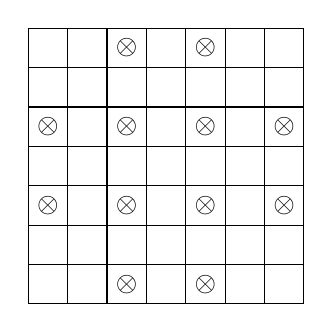
\begin{tikzpicture}
  \foreach \x in {-1.5,-1,-.5,0,.5,1,1.5}
    \foreach \y in {-1.5,-1,-.5,0,.5,1,1.5}
    {
      \draw (\x,\y) +(-.25,-.25) rectangle ++(.25,.25);
    };
    \draw (0,0) node{\textbf{\symknight}};
    \draw (.5,1.5) node{$\otimes$};
    \draw (.5,.5) node{$\otimes$};
    \draw (1.5,.5) node{$\otimes$};
    \draw (-.5,1.5) node{$\otimes$};
    \draw (-.5,.5) node{$\otimes$};
    \draw (-1.5,.5) node{$\otimes$};
    \draw (-.5,-1.5) node{$\otimes$};
    \draw (-.5,-.5) node{$\otimes$};
    \draw (-1.5,-.5) node{$\otimes$};
    \draw (.5,-1.5) node{$\otimes$};
    \draw (.5,-.5) node{$\otimes$};
    \draw (1.5,-.5) node{$\otimes$};
\end{tikzpicture}

% Knight+[2,2]
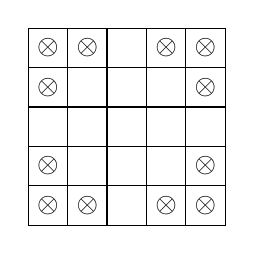
\begin{tikzpicture}
  \foreach \x in {-1,-.5,0,.5,1}
    \foreach \y in {-1,-.5,0,.5,1}
    {
      \draw (\x,\y) +(-.25,-.25) rectangle ++(.25,.25);
      % \draw (\x,\y) node{\symknight};
    };
    \draw (0,0) node{\textbf{\symknight}};
    \draw (.5,1) node{$\otimes$};
    \draw (1,1) node{$\otimes$};
    \draw (1,.5) node{$\otimes$};
    \draw (-.5,1) node{$\otimes$};
    \draw (-1,1) node{$\otimes$};
    \draw (-1,.5) node{$\otimes$};
    \draw (-.5,-1) node{$\otimes$};
    \draw (-1,-1) node{$\otimes$};
    \draw (-1,-.5) node{$\otimes$};
    \draw (.5,-1) node{$\otimes$};
    \draw (1,-1) node{$\otimes$};
    \draw (1,-.5) node{$\otimes$};
\end{tikzpicture}

% Knight+[1,1]
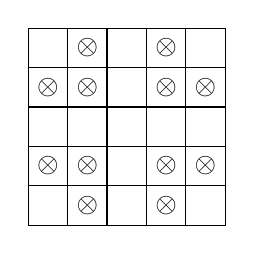
\begin{tikzpicture}
  \foreach \x in {-1,-.5,0,.5,1}
    \foreach \y in {-1,-.5,0,.5,1}
    {
      \draw (\x,\y) +(-.25,-.25) rectangle ++(.25,.25);
      % \draw (\x,\y) node{\symknight};
    };
    \draw (0,0) node{\textbf{\symknight}};
    \draw (.5,1) node{$\otimes$};
    \draw (.5,.5) node{$\otimes$};
    \draw (1,.5) node{$\otimes$};
    \draw (-.5,1) node{$\otimes$};
    \draw (-.5,.5) node{$\otimes$};
    \draw (-1,.5) node{$\otimes$};
    \draw (-.5,-1) node{$\otimes$};
    \draw (-.5,-.5) node{$\otimes$};
    \draw (-1,-.5) node{$\otimes$};
    \draw (.5,-1) node{$\otimes$};
    \draw (.5,-.5) node{$\otimes$};
    \draw (1,-.5) node{$\otimes$};
\end{tikzpicture}

% Knight+[2,0]
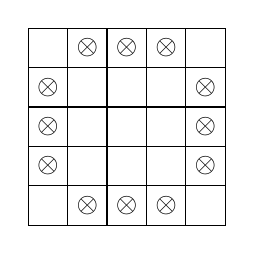
\begin{tikzpicture}
  \foreach \x in {-1,-.5,0,.5,1}
    \foreach \y in {-1,-.5,0,.5,1}
    {
      \draw (\x,\y) +(-.25,-.25) rectangle ++(.25,.25);
      % \draw (\x,\y) node{\symknight};
    };
    \draw (0,0) node{\textbf{\symknight}};
    \draw (.5,1) node{$\otimes$};
    \draw (1,.5) node{$\otimes$};
    \draw (-.5,1) node{$\otimes$};
    \draw (-1,.5) node{$\otimes$};
    \draw (-.5,-1) node{$\otimes$};
    \draw (-1,-.5) node{$\otimes$};
    \draw (.5,-1) node{$\otimes$};
    \draw (1,-.5) node{$\otimes$};
    \draw (1,0) node{$\otimes$};
    \draw (-1,0) node{$\otimes$};
    \draw (0,1) node{$\otimes$};
    \draw (0,-1) node{$\otimes$};
\end{tikzpicture}

% Knight Silver General
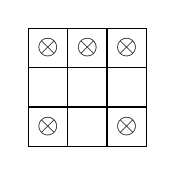
\begin{tikzpicture}
  \foreach \x in {-.5,0,.5}
    \foreach \y in {-.5,0,.5}
    {
      \draw (\x,\y) +(-.25,-.25) rectangle ++(.25,.25);
    };
    \draw (0,0) node{\textbf{\symknight}};
    \draw (.5,.5) node{$\otimes$};
    \draw (0,.5) node{$\otimes$};
    \draw (-.5,.5) node{$\otimes$};
    \draw (.5,-.5) node{$\otimes$};
    \draw (-.5,-.5) node{$\otimes$};
\end{tikzpicture}

% Knight Gold General
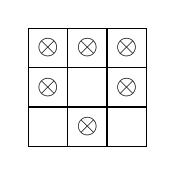
\begin{tikzpicture}
  \foreach \x in {-.5,0,.5}
    \foreach \y in {-.5,0,.5}
    {
      \draw (\x,\y) +(-.25,-.25) rectangle ++(.25,.25);
    };
    \draw (0,0) node{\textbf{\symknight}};
    \draw (.5,.5) node{$\otimes$};
    \draw (-.5,.5) node{$\otimes$};
    \draw (.5,0) node{$\otimes$};
    \draw (-.5,0) node{$\otimes$};
    \draw (0,.5) node{$\otimes$};
    \draw (0,-.5) node{$\otimes$};
\end{tikzpicture}

% Berolina pawn+
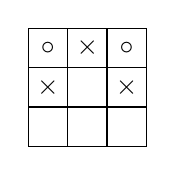
\begin{tikzpicture}
  \foreach \x in {-.5,0,.5}
    \foreach \y in {-.5,0,.5}
    {
      \draw (\x,\y) +(-.25,-.25) rectangle ++(.25,.25);
    };
    \draw (0,0) node{\textbf{\sympawn}};
    \draw (.5,.5) node{$\circ$};
    \draw (-.5,.5) node{$\circ$};
    \draw (.5,0) node{$\times$};
    \draw (-.5,0) node{$\times$};
    \draw (0,.5) node{$\times$};
\end{tikzpicture}

% Berolina pawn
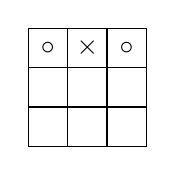
\begin{tikzpicture}
  \foreach \x in {-.5,0,.5}
    \foreach \y in {-.5,0,.5}
    {
      \draw (\x,\y) +(-.25,-.25) rectangle ++(.25,.25);
    };
    \draw (0,0) node{\textbf{\sympawn}};
    \draw (.5,.5) node{$\circ$};
    \draw (-.5,.5) node{$\circ$};
    \draw (0,.5) node{$\times$};
\end{tikzpicture}

% Shogi pawn
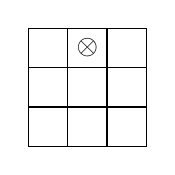
\begin{tikzpicture}
  \foreach \x in {-.5,0,.5}
    \foreach \y in {-.5,0,.5}
    {
      \draw (\x,\y) +(-.25,-.25) rectangle ++(.25,.25);
    };
    \draw (0,0) node{\textbf{\sympawn}};
    \draw (0,.5) node{$\otimes$};
\end{tikzpicture}

\end{document}
